\documentclass{article}

\title{Estatística Numérica Computacional\\Trabalho nº2\\Grupo V}
\author{Marta Paz nº49861\\
		Rafael Almeida nº49788\\
		Rafael Gameiro nº50677\\
		Ricardo Pinto nº49811\\
}
\date{October, 2018}

\usepackage{amsmath}
\usepackage{graphicx}
\usepackage{enumerate}

\begin{document}
	\maketitle
	\pagenumbering{gobble}
	\newpage
	\pagenumbering{arabic}
	
	\section*{Exercício 1}
		\paragraph{}
			Considere as duas amostras de duas v. aleatórias $X$ e $Y$
			
			\begin{table}[!h]
				\begin{tabular}{|c|cccccccc|}
					\hline
 					Amostras de $X$ & 92 & 90 & 85 & 96 & 92 & 88 & 96 & 88 \\
 					\hline
 					Amostras de $Y$ & 89 & 90 & 88 & 93 & 90 & 85 & 95 & 90 \\
 					\hline
				\end{tabular}
			\end{table}
			
			 \begin{enumerate}[(a)]
				\item Use $\hat{\rho} = 
				\frac{\sum_{\substack{i=1}}^{N} (X_i - \bar X)(Y_i - \bar Y)}										{\sqrt{\sum_{\substack{i=1}}^{N}(X_i - \bar X)^2 														\sum_{\substack{i=1}}^{N}(Y_i - \bar Y)^2}}$	
			para estimar o coeficiente de \indent \indent correlação entre as duas variáveis.
			
				\subsection*{Resolução}
					A resolução desta alínea foi feita somente em R.
					
					\begin{figure}[!h]
						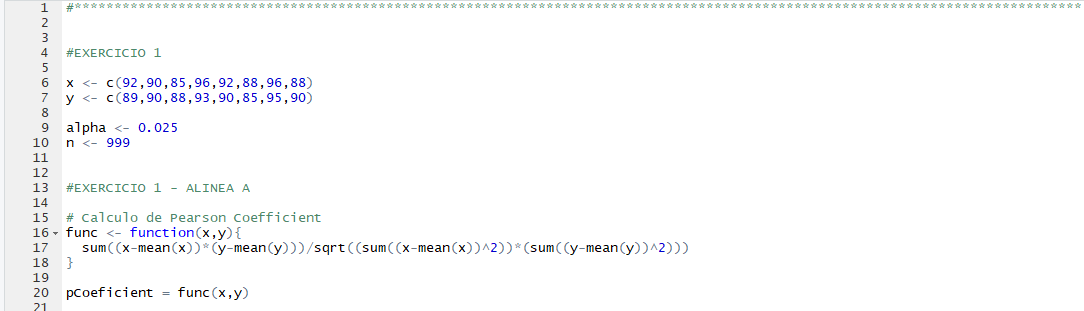
\includegraphics[scale=0.70]{ex1a)}
					\end{figure}

				R: $\hat{\rho} \approx 0.798$
			
				\item Calcule a variância de jackknife de $\hat{\rho}$.
				
				\subsection*{Resolução}	
					Para calcular a variância de jackknife temos a seguinte fórmula:
					
					\begin{equation*}
						Var_{jack} = \frac{1}{n(n-1)}(\sum_{\substack{j=1}}^{N}
									l_{jack}^2 -nb_{jack}^2)
					\end{equation*}		
					
					Para tal, também precisamos de calcular o enviesamento.
					
					\subsubsection*{Definição}
						Suponhamos que	$\rho = t(F)$ e que $F$ é uma função	de distribuição cumulativa e $t(.)$ algo funcional. Então, a função de influência de $t$ em $F$ é dada por:
						
						\begin{equation*}
							L_t(y,F) = \lim_{\varepsilon \to 0} 
							\frac{t\left[(1 - \varepsilon)F + \varepsilon H_y \right] - t(F)}{\varepsilon}
						\end{equation*}	
						e
						\begin{equation*}
							H_y(u) = \begin{cases} 
										0, & u < y\\\\ 1, & u \geq y 
									\end{cases}
						\end{equation*}				
						
						Suponhamos que $x_1, x_2, ..., x_n$ é uma amostra e $\hat{F}$ é uma função empírica da amostra. A função de influência empírica é definida como:
						
						\begin{equation*}
							l(y) = L_t(y, \hat{F})
						\end{equation*}		
						
						Os valores da função de influência empírica nos pontos de dados são chamadas de valores de influência empírica.
						
						\begin{equation*}
							l_j = l(x_j) = L_t(x_j, \hat{F}), \quad j = 1,2,...,n
						\end{equation*}		
						
						Uma extensão do Teorema de Taylor diz que para funções $t$ e 
						medidas $G$ e $F$,
						
						\begin{equation*}
							t(G) \approx t(F) + \int^{}_{} L_t(y,F)dG(y)
						\end{equation*}		
						
						Isto é um resultado exato se $t$ é uma estatística linear.
						Aplicando essa fórmula com $F$ à função de distribuição cumulativa e à função $G = \hat{F}$ obtemos
						
						\begin{align*}
							t(\hat{F}) &\approx t(F) + \int^{}_{} L_t(y,F)d\hat{F}(y) 
							\quad \textrm{,que é}\\
							t(\hat{F}) &\approx t(F) + \frac{1}{n}
										\sum_{\substack{j=1}}^{N} L_t(x_j,\hat{F}) =
										t(F) + \frac{1}{n}\sum_{\substack{j=1}}^{N}l_j\\
							&\Leftrightarrow \rho - \hat{\rho} = -\frac{1}{n}															\sum_{\substack{j=1}}^{N}l_j 
						\end{align*}	
						
						O Jackknife fornece uma maneira de aproximar valores de influência empíricos através da reamostragem dos dados.
						
						\begin{align*}
							L_t(y,F) &= \lim_{\varepsilon \to 0} 
							\frac{t\left[(1 - \varepsilon)\hat{F} + \varepsilon H_y \right] 
							- t(\hat{F})}{\varepsilon}\\
							&\approx  
							\frac{t\left[(1 - \varepsilon)\hat{F} + \varepsilon H_y \right] 
							- t(\hat{F})}{\varepsilon} 
						\end{align*}		 			
						
						Se tomarmos $\varepsilon = \frac{1}{n-1}$, então
						
						\begin{equation*}
							(1 - \varepsilon)\hat{F} + \varepsilon H_{x_j} 
							= \frac{n}{n(n-1)}\hat{F} - \frac{1}{n-1}H_{x_j} = \hat{F}_{-j}
						\end{equation*}
						
						é uma distribuição sem peso no ponto $x_j$ e peso $\frac{1}{n-1}$ no resto da amostra.
						Isto é equivalente a ter apenas a amostra de tamanho $n-1$ encontrada omitindo $x_j$ da amostra original.
						Então, a aproximação Jackknife ao valor da influência empírico $l_j$ é
						
						\begin{equation*}
							l_{jack:j} = (n-1)[t(\hat{F}-t(\hat{F}_{-j}))] = 
							(n-1)(\hat{\rho}-\rho_{-j})
						\end{equation*}
						
						As estimativas imparciais do enviesamento e da variância, que usam os valores de influência empíricos do Jackknife a que chamamos de viés de Jackknife e variância de Jackknife, são:
						
						\begin{align*}
							b_{jack} &= -\frac{1}{n}\sum_{\substack{j=1}}^{N}l_{jack:j}\\
							Var_{jack} &= \frac{1}{n(n-1)}
							(\sum_{\substack{j=1}}^{N}l^2_{jack:j} - nb^2_{jack})
						\end{align*}	

\newpage

						\begin{figure}[!h]
							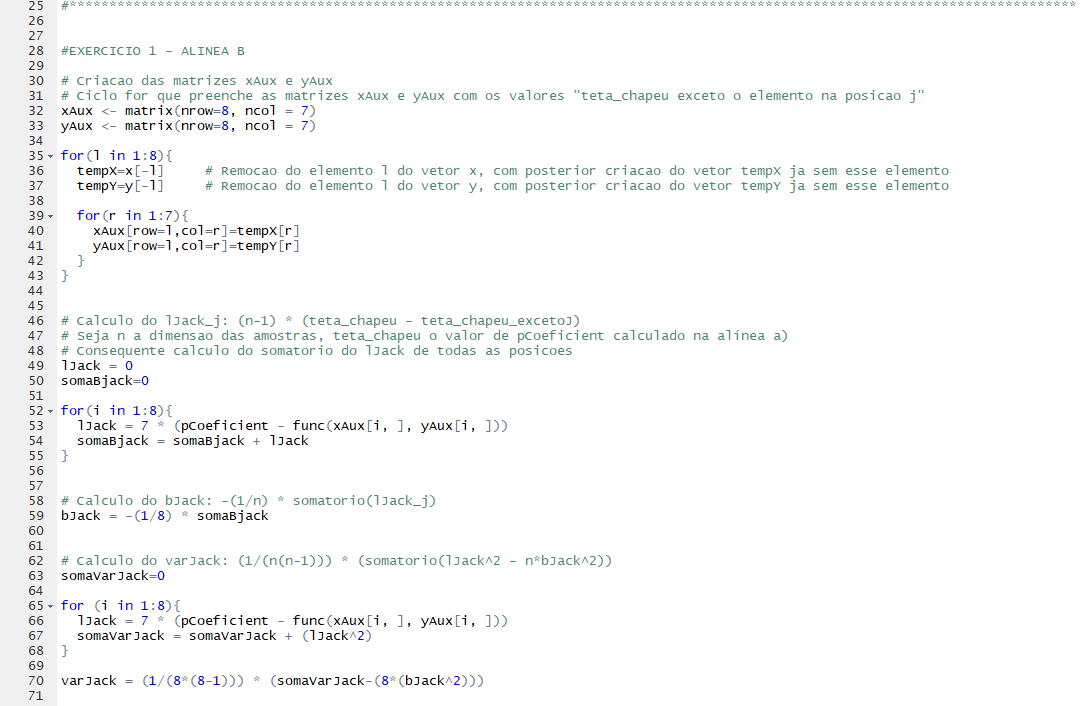
\includegraphics[scale=0.4]{ex1b)}
						\end{figure}

						R: $Var_{jack} \approx 0.014$
				
				\item Construa um intervalo de confiança bootstrap básico para $\rho$.
				
				\subsection*{Resolução}				
				
					Para calcular um intervalo de confiança de Bootstrap tivémos de gerar várias amostras bootstrap, tanto para $X$ como para $Y$. Para tal, aplicámos a cada amostra a fórmula do coeficiente de correlação, e de seguida o enviesamento a cada resultado obtido. Ordenámos os valores e utilizando a estatística pivot,

					\begin{align*}
						\hat{a}_\alpha &= \hat{\rho}_{(R+1).\alpha}^* - \hat{\rho}\\
						\hat{a}_{1 - \alpha} &= \hat{\rho}_{(R+1).(1 - \alpha)}^* - \hat{\rho}
					\end{align*}	

					obtivémos o intervalo de confiança na forma,

					\begin{equation*}
							]\hat{\rho} - \hat{a}_{1 - \alpha}, \hat{\rho} - \hat{a}_\alpha [
					\end{equation*}	

\newpage

					\begin{figure}[!h]
						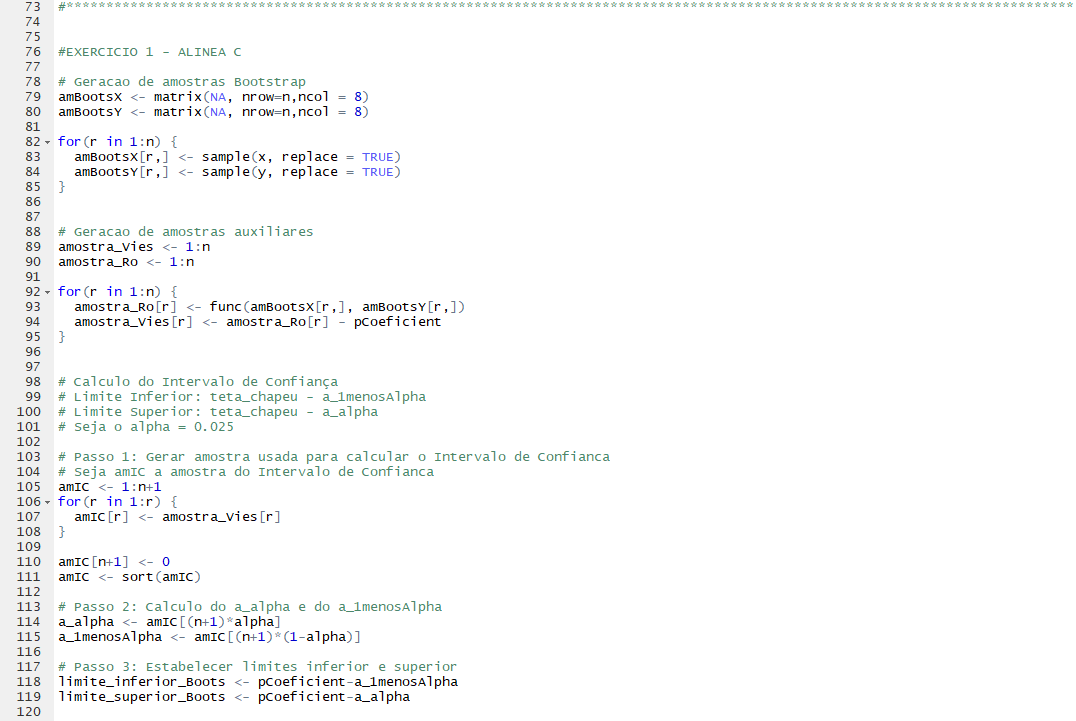
\includegraphics[scale=0.4]{ex1c)}
					\end{figure}

					R: $]0.86, 2.33[$

				\item Construa um intervalo de confiança t-bootstrap para $\rho$. Use a variância bootstrap para estimar a variância de $\hat{\rho_r}^*$.
				
				\subsection*{Resolução}	

					Para o cálculo do intervalo de confiança bootstrap studentized utilizámos uma estatística pivot diferente da usada no cálculo do bootstrap básico:

					\begin{align*}
						&\hat{z} = \frac{\hat{\rho}^* - \hat{\rho}}																	{\sqrt{Var_{Boots}(\hat{\rho}^*)}}\\\\
						&Var_{Boots}(\hat{\rho}^*) = \frac{1}{n-1}\sum_{\substack{j=1}}^{N}											(\hat{\rho_j}^* - \bar{\hat{\rho}}^*)^2
					\end{align*}	
					
\newpage
					
					Primeiramente, usámos as amostras bootstrap geradas da alínea c) para o cálculo dos $\hat{\rho_r}^*$. Para obtermos a variância bootstrap de cada $\hat{\rho_r}^*$, gerámos um novo conjunto de amostras bootstrap com base em cada amostra previamente usada na alínea anterior.\\
				    O resto do procedimento, foi a reordenação dos diferentes valores de $z$, e a determinação do intervalo de confiança, usando a fórmula

					\begin{equation*}												
							]\hat{\rho} - \hat{z}_{(R+1)(1 - \alpha)}^*\sqrt{Var_{Boots}(\hat{\rho})}, \hat{\rho} - \hat{z}_{(R+1)(\alpha)}^*\sqrt{Var_{Boots}(\hat{\rho})} [
					\end{equation*}	

					\begin{figure}[!h]
						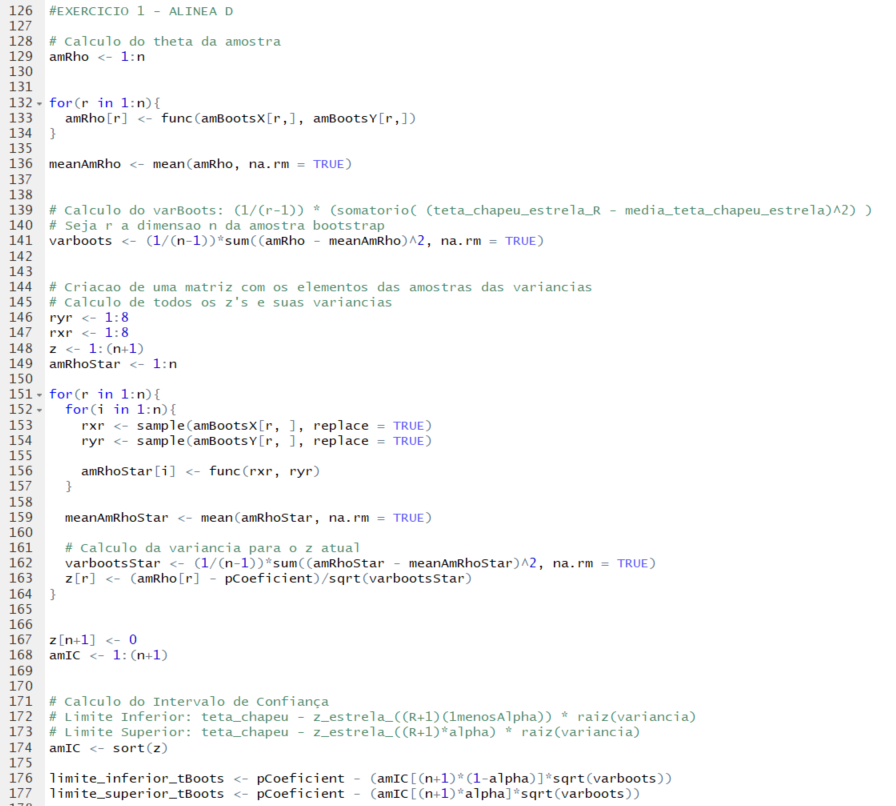
\includegraphics[scale=0.6]{ex1d)}
					\end{figure}

					R: $]0.89,  2.27[$
					
\newpage
	
					\subsection*{Discussão}
	
						\paragraph*{}
							 Comparativamente com o método Bootstrap, o método Jackknife é mais rápido a executar e permite calcular estatísticas não-paramétricas. Por outro lado, uma vez que o intervalo de confiança baseia-se em aproximações, o melhor método a ser usado é o de Bootstrap.\\ 
					
						\paragraph*{}
							O intervalo de confiança bootstrap studentized tem menor amplitude que o intervalo de confiança bootstrap básico. Uma vez que quanto menor for a amplitude de um intervalo, maior será a sua precisão, então podemos concluir que o intervalo de confiança bootstrap studentized é mais preciso que o de bootstrap básico.
							O intervalo de confiança bootstrap básico não se encontra como seria esperado, pois o valor $\rho$ calculado anteriormente não pertence a esse intervalo.
							O intervalo de confiança bootstrap studentized também não está como era esperado, pois o valor $\rho$ calculado anteriormente não pertence a esse intervalo. 	
				
			\end{enumerate}		
				
	\section*{Exercício 2}
		\paragraph{}
			Considere a amostra seguinte:
			
			\begin{table}[!h]
				\begin{tabular}{|c|c|c|c|c|c|c|c|c|c|c|c|c|c|c|c|c|c|c|c|}
					\hline
 					1 & 3 & 3 & 1 & 1 & 3 & 2 & 2 & 3 & 0 & 2 & 4 & 2 & 6 & 4 & 2 & 4 & 3 & 2 & 4\\
 					\hline
				\end{tabular}
			\end{table}
			
			\noindent Considere a hipótese nula, $H_0$ : A v.a. subjacente a esta amostra tem distrbuição binomial de parâmetros $(8, 0.3)$. Use a função de distribução empírica da estatística de teste para estimar o $p-value$ da estatística de teste qui-quadrado, $T$ que permite testar a hipótese nula.
			
			\begin{equation*}
				T = \sum_{\substack{i=1}}^{k} \frac{(N_i - np_i)^2}{np_i}
			\end{equation*}
			
			
			\indent\indent\indent\indent\indent $i \in \{1,...,K\}$ - suporte da v.a.\\
			\indent\indent\indent\indent\indent$\{p_i,i=1,...,K\}$ - função de probabilidade da v.a.\\
			\indent\indent\indent\indent\indent$n$ - dimensão da amostra.\\
			\indent\indent\indent\indent\indent$N_i$ - número de observações na amostra que tomam o valor $i$.\\
			
\newpage
			
			\subsection*{Resolução}
			
				Neste exercício, foi-nos dada uma amostra e a seguinte hipótese nula:\\\\
				\indent $H_0$: A variável aleatória subjacente a esta amostra tem distribuição binomial de parâmetros $(8, 0.3)$.\\
				
				De seguida, era pedido que usássemos a função de distribuição empírica da estatística de teste para estimar o $p-value$ da estatística de teste qui-quadrado, $T$, que permite testar a hipótese nula fornecida.\\
				Desta forma, para o teste de hipótese que realizámos, cosiderámos as seguintes hipóteses:\\\\
				\indent $H_0$: A variável aleatória subjacente a esta amostra tem distribuição binomial de parâmetros $(8, 0.3)$.\\\\
				\indent $H_1$: A variável aleatória subjacente a esta amostra não tem distribuição binomial de parâmetros $(8, 0.3)$\\
				

				Para calcular o valor do p-value, utilizámos a seguinte fórmula:

			 	\begin{equation*}
					p-value = \hat{P}(T > t_{obs}|H_0) = 1 - \hat{F}_{H_0}(t_{obs}) =
							\frac{\# \left \{ t_j : t_j \geq t_{obs} \right \} + 1}{m + 1}
				\end{equation*}
				
				Para podermos utilizar a fórmula acima, tivemos de calcular os seguintes valores:
				\begin{enumerate}
					\item $t_{obs}$, que corresponde ao valor da estatística de teste dos valores observados (valores estes que foram dados no enunciado). Recorremos à seguinte fórmula para o cálculo da estatística de teste (que foi dada no enunciado do problema): 
				
				\begin{equation*}
					T = \sum_{\substack{i=1}}^{k} \frac{(N_i - np_i)^2}{np_i}
				\end{equation*}
				
				E  realizámos os seguintes passos no R:
				
				\begin{enumerate}
				 	\item Percorremos a amostra dada no enunciado e contámos o número de ocorrências de cada elemento (0 a 6, pois a amostra só tem elementos compreendidos entre esses valores). Para guardar o número de ocorrências usámos um vetor, nObs, em que cada posição correspondia a um valor do intervalo entre 0 e 6. 
				 	\item Fizémos um ciclo onde é calculado a probabilidade binomial, com os parâmetros fornecidos, de cada ocorrência.
				 	\item Por último, aplicámos a fórmula da estatística de teste acima ao conjunto das probabilidades calculadas no ponto anterior e daqui obtivémos que $t_{obs} = 2.205978$.
				\end{enumerate}
				 
					\item $t_j$, que corresponde ao valor da estatística de teste assumindo que a hipótese nula é verdade. Para tal, criámos uma matriz, amAux, onde cada linha vai corresponder a uma amostra gerada com o comando \textit{rbinom} do R usando os parâmetros da distribuição binomial que nos deram no enunciado.\\
						De seguida criámos uma matriz, nObsAux, onde guardámos o número de ocorrências decada, em cada amostra gerada.
						Depois, calculámos a probabilidade de cada posição de nObsAux acontecer e, com os valores obtidos, pudémos calcular os $t_j$'s. Para cada $t_j$, comparámos o seu valor com $t_obs$ e contámos quantas vezes $t_j$ era igual ou superior que $t_{obs}$. Esse valor foi guardado na nossa variável $soma$. 
				 	\item Por último, aplicámos a fórmula do $p-value$ aos valores que obtivémos, ou seja:

						\begin{equation*}
							p-value = \frac{soma + 1}{(999 + 1) + 1}\approx 0.86
						\end{equation*}
				
				\end{enumerate}
				Para verificar se aceitamos a hipótese nula, considerámos três valores diferentes para o nivel de significância: $\alpha = 0.01$,  $\alpha = 0.025$ e $\alpha = 0.5$. 

				\noindent Para os três valores de alfa considerados, verificámos que $p-value \geq \alpha$, logo não rejeitamos a hipótese nula nos três níveis de significância. Isto é, existem evidências estatísticas para afirmar que a variável aleatória subjacente à amostra fornecida tem distribuição binomial de parâmetros $(8, 0.3)$.
				
\newpage			
			
				\begin{figure}[!h]
					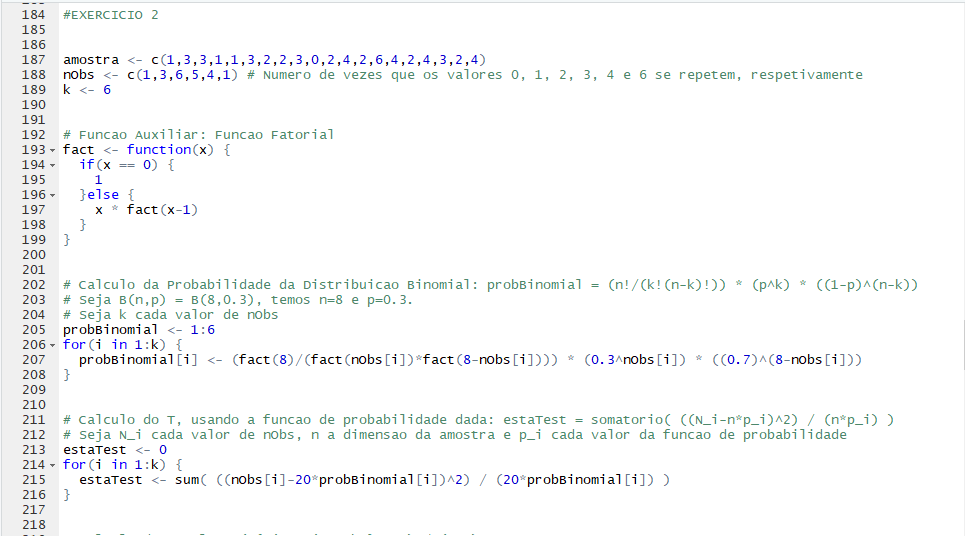
\includegraphics[scale=0.45]{oi}
				\end{figure}
				\begin{figure}[!h]
					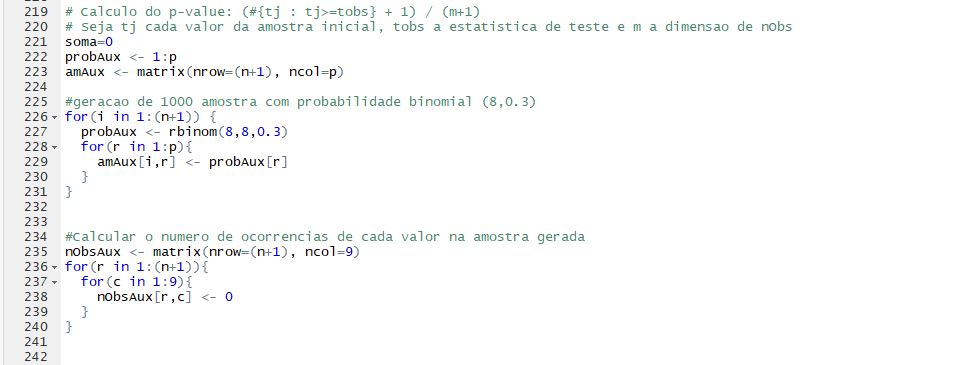
\includegraphics[scale=0.45]{oi2}
				\end{figure}
				
\newpage				
				
				\begin{figure}[!h]
					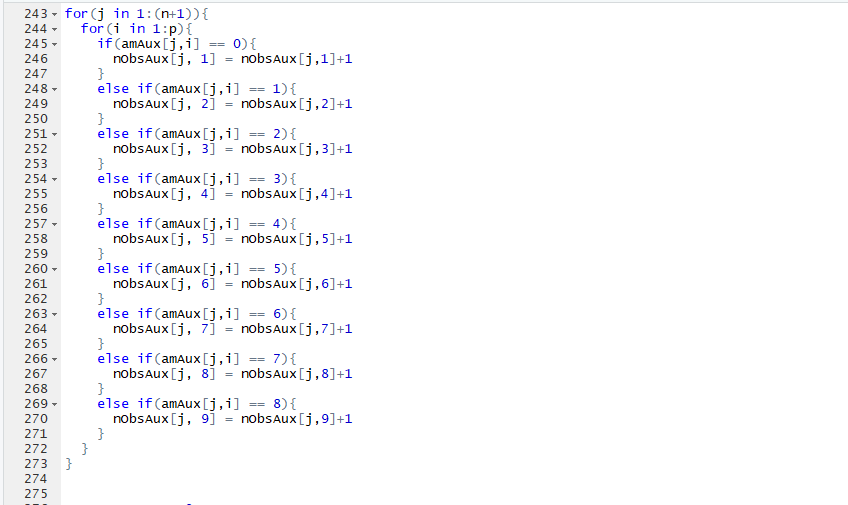
\includegraphics[scale=0.45]{oi3}
				\end{figure}
				\begin{figure}[!h]
					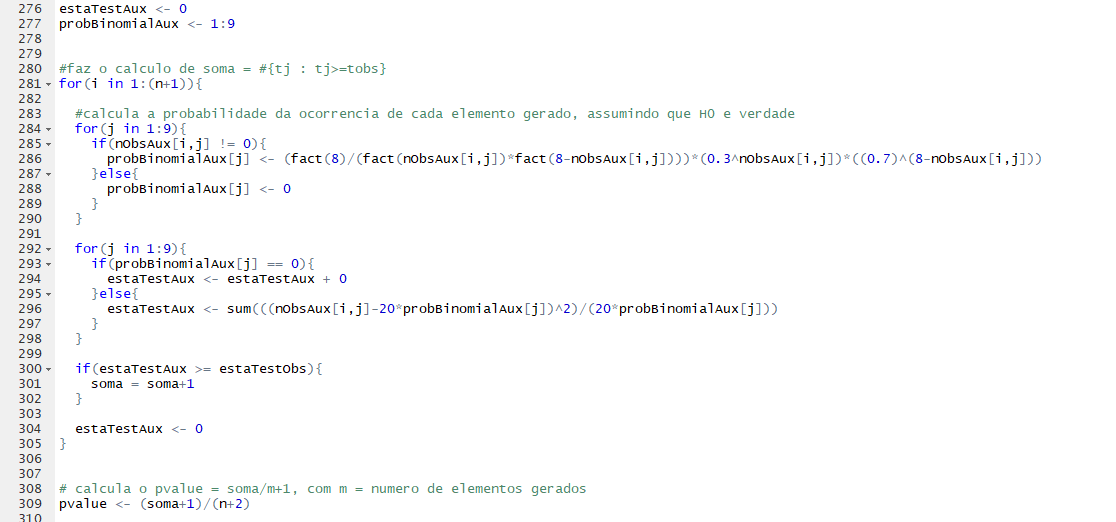
\includegraphics[scale=0.45]{oi4}
				\end{figure}
			
\end{document}
